\documentclass{article}
\usepackage[utf8]{inputenc}

\usepackage{times}
\usepackage{graphicx}
\usepackage{amsmath}
\usepackage{amsfonts}
\usepackage{amssymb}
\usepackage{color, soul}
\usepackage{natbib} 

\renewcommand{\vec}[1]{\boldsymbol{{#1}}} 

\title{The Climate Machine (CLIMA)}
\author{Climate Modeling Alliance}

\begin{document}

\maketitle

\section{Overview}

To achieve a step change in the accuracy and precision of climate simulations and predictions, we are developing CLIMA, an Earth system model (ESM) that learns automatically from diverse data sources. Our goal is to use observational data along with modern computational methods not simply to evaluate and test models, as is current practice, but to systematically reduce model-data mismatches and quantify uncertainties. To accomplish this goal, we will harness, simultaneously and self-consistently, orders-of-magnitude more data than are currently used in model development, exploiting new techniques from data assimilation (DA) and machine learning (ML).

\subsection{Automated Learning From Observations and High-Resolution Simulations}

We will design an ESM platform with subgrid-scale (SGS) process models that learn automatically from two sources of information (for more details and references, see \citet{Schneider17c}, from which several passages of this document are taken):
\begin{enumerate}
    \item \emph{Global observations.} We live in the golden age of Earth observations from space. A suite of satellites is streaming coordinated and nearly simultaneous measurements of variables such as temperature, humidity, clouds, ocean surface currents, and sea ice cover, with global coverage for more than a decade. Space-based measurements of biogeochemical tracers and processes, such as measurements of column-average CO2 concentrations, of ocean biomass, and of photosynthesis in ecosystems, are also available, and so are more detailed observations of the cryosphere. To date, only a minute fraction of the data (mostly large-scale energy fluxes) has been directly used in ESM development (as opposed to ESM evaluation). CLIMA will learn directly from global data, augmented and validated with more detailed local observations where available.
    \item \emph{Local high-resolution simulations.} Some SGS processes in ESMs are in principle computable, only the globally achievable resolution precludes their explicit computation. For example, the turbulent dynamics of clouds can be computed with high fidelity in limited domains in large-eddy simulations (LES) with mesh sizes of meters to tens of meters. Increased computational performance has made LES domain widths of 10--100~km feasible in recent years, while the horizontal mesh size in climate models has shrunk, to the point that the two scales have converged \citep{Schneider17a}. Thus, while global LES that reliably resolve low clouds will not be feasible for decades, it is now possible to nest LES in limited areas of atmosphere models and conduct targeted local high-fidelity simulations of cloud dynamics in them. Local high-resolution simulations of ocean turbulence or sea ice dynamics can be conducted similarly. CLIMA will learn from such nested high-resolution simulations.
\end{enumerate}
Simultaneously exploiting global observations and local high-resolution simulations with new DA/ML tools presents the key opportunity for  progress in Earth system modeling. Replacing the inefficient and sub-optimal manual tuning process and the offline fitting of parameterization schemes to data from few locations, as is currently common, CLIMA will autotune itself and quantify its uncertainties based on statistics of much larger range of available data. It will adapt as new observations come online, and it will generate targeted high-resolution simulations on the fly---akin to targeted observations in weather forecasting \citep{Palmer98a,Lorenz98a}---to reduce and quantify uncertainties where needed to tighten estimates of SGS models of computable processes. This will increase the amount of data to which SGS models are fitted by several orders of magnitude.

\subsection{Optimization Over Aggregate Climate Statistics}

The automated learning from observations and high-resolution simulations in CLIMA will use \emph{statistics accumulated in time} (e.g., over seasons) to:
\begin{enumerate}
\item Minimize model biases, especially biases that are known to correlate with the climate response of models. This amounts to minimizing mismatches between time averages of ESM-simulated quantities and data.
\item Minimize model-data mismatches in higher-order Earth system statistics. This includes covariances such as cloud-cover/surface temperature covariances, or ecosystem carbon uptake/surface temperature covariances, which are known to correlate with the climate response of models (``emergent constraints''). It can also include higher-order statistics involving direct targets for prediction goals, such as rainfall extremes. 
\end{enumerate}
By optimizing how well an ESM simulates climate statistics, our approach directly targets success metrics that are relevant for climate projections. Optimizing over climate statistics ameliorates problems arising from ill-posedness of the inverse problem (underdetermination of SGS models given data), and it  avoids difficulties caused by sensitive dependences on atmospheric initial conditions and small-scale roughness. These difficulties arise when optimizing over snapshots of Earth system states, as in numerical weather prediction. For example, the challenge of simulating when and where clouds occur, with temporal and spatial accuracy (e.g., hours to minutes in time and kilometers to hundred meters in space), has prevented the routine assimilation of space-based radar and lidar observations of clouds in numerical weather predictions \citep{Stephens18a}. But if these same data are aggregated, for example, over seasons, precisely when and where individual clouds occur, and their sensitive dependence on atmospheric initial conditions, become less important. The aggregated cloud statistics vary smoothly in time and space, and minimizing mismatches in them directly targets what matters for climate projections. This is where the key untapped opportunity lies for CLIMA to radically improve upon existing models.

The problem of minimizing model-data mismatches in climate statistics is computationally challenging because accumulating statistics from an ESM is costly: each evaluation of the target statistics requires an ESM simulation at least over a season. But the computational problems are just beginning to be tractable, for example, with the ensemble-based inversion methods we will develop and employ.

\subsection{Computable and Noncomputable Parameters}

Learning from  local high-resolution simulations and observations is aimed at determining two different kinds of parameters in parameterization schemes: \emph{computable} and \emph{non-computable} parameters. (Since parameters and parametric functions of state variables play essentially the same role in our discussion, we simply use the term parameter, with the understanding that this can include parametric functions and even nonparametric functions.) Computable parameters are those that can in principle be inferred from high-resolution simulations alone. They include parameters in radiative transfer schemes, which can be inferred from detailed line-by-line calculations; dynamical parameters in cloud turbulence parameterizations, such as entrainment rates, which can be inferred from LES; or parameters in ocean mixing parameterizations, which can be inferred from high-resolution simulations. Non-computable parameters are parameters that, currently, cannot be inferred from high-resolution simulations, either because computational limitations make it necessary for them to also appear in parameterization schemes in high-resolution simulations, or because the microscopic equations governing the processes in question are unknown. They include parameters in cloud microphysics parameterizations, which are still necessary to include in LES, and many parameters characterizing ecological and biogeochemical processes, whose governing equations are unknown. Cloud microphysics parameters will increasingly become computable through direct numerical simulation, but ecological and biogeochemical parameters will remain non-computable for the foreseeable future. We will denote computable parameters by $\vec{\theta}_c$ and non-computable parameters by $\vec{\theta}_n$. Jointly, they form the parameter vector $\vec{\theta}=(\vec{\theta}_c, \vec{\theta}_n)$.

Both computable and non-computable parameters can, in principle, be learned from observations; the only restrictions to their identifiability come  from the well-posedness of the learning problem and its computational tractability. But only computable parameters can be learned from targeted high-resolution simulations. To be able to learn computable parameters, it is essential to represent non-computable aspects of a parameterization scheme consistently in the high-resolution simulation and in the parameterization scheme that is to learn from the high-resolution simulation. For example, radiative transfer and microphysical processes need to be represented consistently in a high-resolution LES and in a parameterization scheme if the parameterization scheme is to learn computable dynamical parameters such as entrainment rates from the LES. 

\subsection{Fresh Model Architecture}

\begin{figure}
\centerline{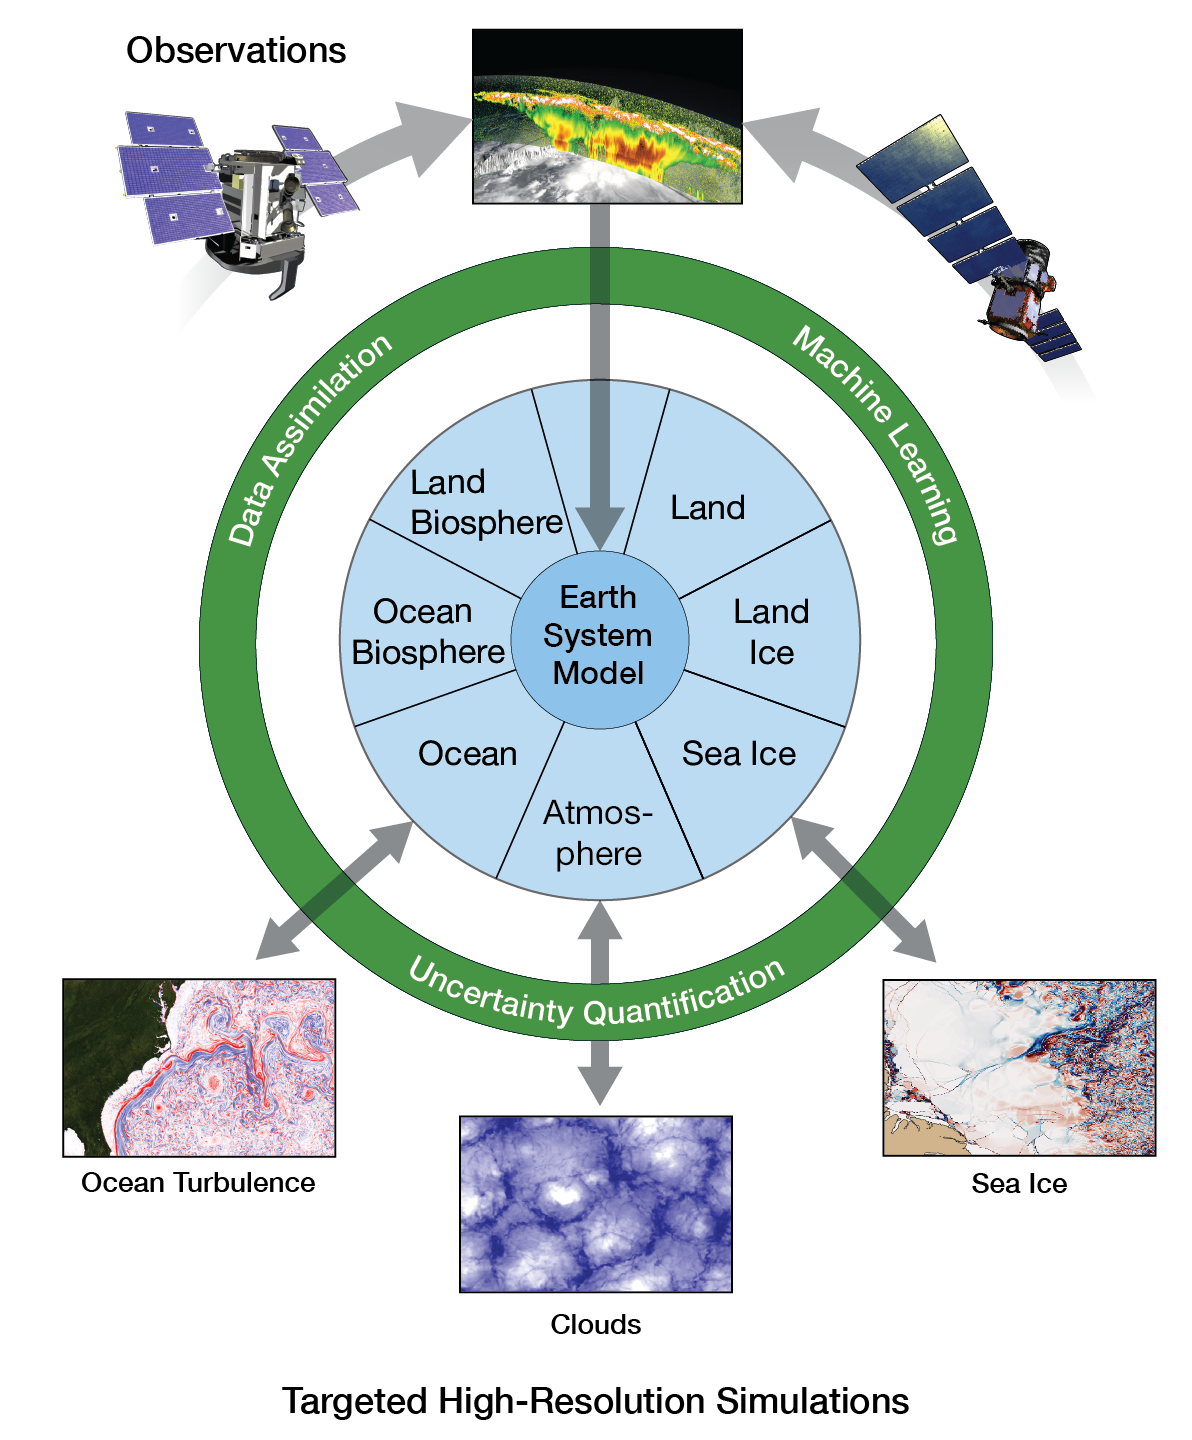
\includegraphics[width=.95\textwidth]{CLIMA-schematic.png}}
\caption{\textbf{Schematic of CLIMA.} Observations of the Earth system (e.g., from space) and output from targeted high-resolution simulations (e.g., of ocean turbulence) are passed through a data assimilation/machine learning (DA/ML) layer, which wraps around an Earth system model (ESM) with its component models. The high-resolution simulations that inform the ESM through the DA/ML layer are spun off from component models such as the atmosphere or ocean models. The DA/ML layer not only optimizes the ESM components but also quantifies uncertainties about model processes.} 
\label{f:CLIMA-schematic}
\end{figure}
CLIMA will have a fresh model architecture (see the schematic in Fig.~\ref{f:CLIMA-schematic}). Current ESM architectures make it difficult to carry out the hundreds to thousands of ESM simulations that are necessary for DA/ML based on climate statistics, and current parameterization schemes are not well suited for DA/ML approaches (e.g., because they contain many correlated parameters).  We will need to design CLIMA to learn efficiently from observations and to run nested high-resolution simulations on the fly, and we will need to replace several existing parameterization schemes by flexible SGS process models that learn effectively from diverse data sources. The SGS process models need to be systematically refine-able as more data become available, and they need to treat subgrid-scale motions (e.g., boundary layer turbulence, shallow convection, deep convection) in a unified manner. Achieving this will be a central focus of our development effort.

To achieve rapid payoffs in terms of reduced uncertainties in climate projections, we will focus the early development on the most uncertain components for which we have already begun development and prototyping of new SGS process models (e.g., for clouds, convection, and turbulence), while initially using other components from existing models. However, we will eventually seek to replace most current parameterization schemes by more flexible SGS process models designed for DA/ML approaches. 

To be fast and run at the highest resolutions feasible, CLIMA will also need to effectively exploit the computing architectures that are currently emerging, including heterogeneous many-core architectures that combine traditional CPUs with hardware accelerators such as graphical processing units (GPUs) or Field Programmable Gate Arrays (FPGAs). Targeted high-resolution simulations nested in a global ESM are ideally suited for running on accelerators, which shine at solving computational problems that can be decomposed into largely independent subtasks that are comparable in computational effort. Many high-resolution simulations---potentially hundreds or thousands---can be run concurrently with the coarse-resolution ESM, avoiding idle computational threads that otherwise limit accelerator efficiency. We may also want to exploit emerging AI accelerator designs, when they are broadly available, in the DA/ML components of the ESM platform.

\section{CLIMA Layers and Goals}

CLIMA consists of several layers (Fig.~\ref{f:CLIMA-schematic}). Wrapped around what traditionally would be the ESM is a DA/ML layer, whose function it is to connect the ESM with observations and targeted high-resolution simulations, to learn about uncertain SGS processes in the ESM. For example, the DA/ML layer allows the ESM to learn about uncertain SGS models of ocean turbulence through matching simulated statistics of ocean turbulence to those observed by satellite altimeters. Or, the DA/ML layer allows the ESM to learn about uncertain SGS models of clouds, convection, and atmospheric turbulence through matching ESM-simulated statistics of cloud cover and cloud condensate to those obtained from LES spun-off from the atmosphere model.

To design CLIMA to learn from diverse data sources, we will employ the key concepts and pursue the goals described in what follows, moving layerwise from the outside to the computational core.

\subsection{Observations}

\paragraph{Concepts}
\begin{itemize}
    \item Observations are primarily space-based or ground-based observations with large spatial coverage.
    \item Observations can also come from field campaigns, which provide more detailed data that are local in space and time. It remains to be seen whether we want to learn from such local data online in CLIMA, or whether we primarily want to use local data in off-line development and testing of SGS models and to provide prior information for learning in CLIMA.
    \item Observables $\vec{y}$ are linked to state variables $\vec{x}$ of the ESM through a map $\mathcal{H}$ representing an observing system, so that 
    \begin{equation}
    \vec{y}(t)=\mathcal{H}\bigl(\vec{x}(t)\bigr).
    \end{equation}
    The observables $\vec{y}$ might represent surface temperatures, cloud cover, or spectral radiances emanating from the TOA. The map $\mathcal{H}$ projects ESM state variables $\vec{x}$ to observables at the locations and times at which actual observations, denoted by $\vec{\tilde y}$, are available. For complex observing systems (e.g., satellites), the map $\mathcal{H}$ represents an observing system simulator and hence can be complicated.
\end{itemize}

\paragraph{Goals}
\begin{itemize}
    \item For the atmosphere, focus first on learning from reanalysis data, including seasonally and spatially varying statistics of variables such as atmospheric temperature and precipitation for the satellite era (from 1980 onward). Reanalyses provide easily accessible and homogenized data, for which the map $\mathcal{H}$ is a simple projection operator. This will allow us to prototype and develop the CLIMA platform more quickly than would be possible if we were to integrate a large set of diverse observational data sources from the outset, which each requires a separate observing system simulator $\mathcal{H}$.
    \item For the ocean, focus first on \hl{[what precisely is our goal here? Ocean measurements from campaigns such as DIMES, Latmix, and OSMOSIS? ECCO?]}
    \item As soon as possible, incorporate selected satellite data products where reanalysis data do not provide adequate information about uncertain SGS processes. Initially, this will likely include cloud data products from platforms such as CloudSat, CALIPSO, and MODIS.
    \item Over time (likely years 4--5), incorporate other observations (e.g., satellite data products) in CLIMA. 
\end{itemize}

\subsection{Targeted High-Resolution Simulations}

\paragraph{Concepts}
\begin{itemize}
    \item Local high-resolution simulations can provide information about uncertain computable parameters $\vec{\theta}_c$ in SGS processes where observations alone do not provide sufficient information about them. This can include high-resolution simulations of atmospheric clouds, convection, and turbulence, of ocean turbulence both on the mesoscale and submesoscale, and of sea ice dynamics. 
    \item Local high-resolution simulations are nested within small areas of the respective ESM component models. For example, atmospheric LES are spun off from the atmosphere model component, nested in small areas (e.g., a grid column) of the global model. Ocean mesoscale-resolving simulations are spun off from the ocean model, in ocean patches that represent a small fraction of the globe, yet are large enough that nonlocal effects (e.g., advection by low-frequency flow components) can be meaningfully represented.
    \item One-way nesting suffices for the high-resolution simulations, simplifying the embedding of the high-resolution simulations. That is, the global component model drives local high-resolution simulations, but the high-resolution simulations do not directly feed back onto the global model (except through the information they provide on SGS models).
    \item Conceptually, local high-resolution simulations may be viewed as a time-depen\-dent map $\mathcal{L}$ from ESM state variables $\vec{x}$  to simulated state variables $\vec{\tilde z}$,
    \begin{equation}
    \vec{\tilde z}(t) = \mathcal{L}(\vec{\theta}_n,t; \vec{x}).
    \end{equation}
    The map $\mathcal{L}$ is parameterized by time $t$ and by parameters $\vec{\theta}_n$ that are not computable in the high-resolution simulation and are inherited from the global model (e.g., microphysical parameters in an atmospheric LES). The map $\mathcal{L}$ can involve the time-history of the state variables $\vec{x}$ up to time $t$, e.g., as time-evolving large-scale boundary condition for the high-resolution simulation. 
    \item The vector of simulated state variables $\vec{\tilde z}$ contains high-resolution variables aggregated over grid boxes of the global model,  such as the mean cloud cover or liquid water content in a grid box. Their counterparts in the global model are computed by parameterization schemes.
    \item The corresponding variables $\vec{z}$ in the global model are obtained by a time-depen\-dent map $\mathcal{S}$ that takes state variables $\vec{x}$ and parameters $\vec{\theta} = (\vec{\theta}_c, \vec{\theta}_n)$ to $\vec{z}$,
    \begin{equation}
    \vec{z}(t) = \mathcal{S}(\vec{\theta},t; \vec{x}).
    \end{equation}
    The map $\mathcal{S}$ typically represents a single grid column of the ESM with its parameterization schemes, taking as input $\vec{x}$ from the ESM. It is structurally similar to $\mathcal{L}$. Mismatches between $\vec{z}$ and $\vec{\tilde z}$ can be used to learn about computable parameters $\vec{\theta}_c$ because $\vec{\tilde z}$ does not depend on them.
    \item The high-resolution simulated state variables $\vec{\tilde z}$ can also be compared to observations $\vec{\tilde y}$. To do so, a map $\mathcal{Z}$ takes high-resolution simulated state variables to observables,
    \begin{equation}
        \vec{y}(t) = \mathcal{Z}\bigl(\vec{\tilde z}(t)\bigr),
    \end{equation}
    e.g., cloud condensate amounts from LES to observable cloud condensate amounts. Mismatches between observables $\mathcal{Z}(t, \vec{\tilde z})$ and actual observations $\vec{\tilde y}$ can be used to learn about non-computable parameters $\vec{\theta}_n$ because high-resolution simulated state variables $\vec{\tilde z}$ depend on the non-computable parameters, but the observations $\vec{\tilde y}$ do not. 
    \item  Models of non-computable processes in the high-resolution simulation $\mathcal{L}$ and in the single-column model $\mathcal{S}$ need to be represented consistently, so that the non-computable processes in $\mathcal{S}$ are a consistently coarse-grained version of those in $\mathcal{L}$. This is necessary to be able to learn about the computable parameters $\vec{\theta}_c$ without the aliasing errors that would arise if non-computable processes are represented inconsistently across the hierarchy. It is also necessary to be able to use mismatches between $\mathcal{Z}(t, \vec{\tilde z})$ and observations $\vec{\tilde y}$ to learn about non-computable parameters $\vec{\theta}_n$ both in the ESM component model and in the high-resolution model.
\end{itemize}

\paragraph{Goals}
\begin{itemize}
    \item Design the high-resolution simulations to run efficiently on accelerators and in distributed computing environments.  For example, it may be desirable to have one high-resolution simulation per GPU. But more flexible layouts (e.g., one high-resolution simulation spread over several GPUs) should also be possible.
    \item Represent non-computable processes in the ESM component models (e.g., microphysics in atmosphere model) and in the high-resolution simulations (e.g., microphysics in atmospheric LES) consistently. That is, the non-computable process models in the ESM need to be consistently coarse-grained version of those in the high-resolution simulations, and the high-resolution simulations need to inherit the non-computable parameters $\vec{\theta}_n$ from the global model.
    \item Target a vertical resolution in atmospheric LES of about 10~m or finer, and a horizontal resolution of 50~m or finer. These are the minimum resolutions necessary to begin to resolve the challenging dynamics of stratocumulus clouds. 
    \item \hl{Ocean}
    \item Make it easily addressable from the DA/ML layer at which physical locations high-resolution simulations are nested in the global model, to be able to target high-resolution simulations where they have the greatest impact on uncertainty reduction. 
\end{itemize}

\subsection{DA/ML Layer}

\paragraph{Concepts}
\begin{itemize}
    \item The DA/ML layer implements the algorithms for learning about parameters (and parameteric functions) $\vec{\theta}$, both from observations and from targeted high-resolution simulations. It sits at the interface of models and data and combines both. It also targets high-resolution simulations where they are impactful in reducing uncertainties about parameters. 
    \item From the perspective of the DA/ML layer, the ESM is a function $\mathcal{G}$, parameterized by time $t$, that maps parameters $\vec{\theta}$ characterizing uncertain processes to climate state variables $\vec{x}$:
    \begin{equation}
    \vec{x}(t) = \mathcal{G}(\vec{\theta}, t).
    \end{equation}
    The state variables $\vec{x}$ can include temperatures, humidity variables, and cloud, cryosphere, and biogeochemical variables, and the map $\mathcal{G}$ may depend on initial conditions and time-evolving boundary or forcing conditions. The vector of parameters $\vec{\theta}$ can include traditional parameters in SGS models, parameters appearing in parametric functions in SGS models about which we want to learn from data, or parameters characterizing nonparametric functions in SGS models, such as Gaussian process models \citep{Kennedy01a,OHagan06a}.  
    \item The map $\vec{y}(t)=\mathcal{H}\bigl(\vec{x}(t)\bigr)$ takes ESM state variables $\vec{x}$ to observables $\vec{y}$. Because $\vec{y}$ is parameterized by $\vec{\theta}$, while the actual observations $\vec{\tilde y}$ are independent of the parameters $\vec{\theta}$, mismatches $\vec{y} - \vec{\tilde y}$ can be used to learn about the uncertain parameters $\vec{\theta}$. 
    \item Similarly, the map $\vec{z}(t) = \mathcal{S}(\vec{\theta},t; \vec{x})$ (a single-column model) takes state variables $\vec{x}$ to variables $\vec{z}$ computable in high-resolution simulations $\mathcal{L}$. Crucially, the map $\mathcal{S}$ generally depends on all parameters $\vec{\theta}=(\vec{\theta}_c, \vec{\theta}_n)$, while $\mathcal{L}$ only depends on non-computable parameters $\vec{\theta}_n$. Thus, mismatches $\vec{z}(t) - \vec{\tilde z}(t)$ can be used to learn about the computable parameters $\vec{\theta}_c$.
    \item Additionally, the map $\vec{y}(t) = \mathcal{Z}\bigl(\vec{\tilde z}(t)\bigr)$ takes high-resolution state variables $\vec{\tilde z}$ to observables $\vec{y}$. Because $\vec{\tilde z}$ is parameterized by non-computable parameters $\vec{\theta}_n$, mismatches $\mathcal{Z}\bigl(\vec{\tilde z}(t)\bigr) - \vec{\tilde y}$ can be used to learn about the non-computable parameters $\vec{\theta}_n$.
    \item Objective functions are defined using time-averaged statistics. We denote the time average of a function $\phi(t)$ over the time interval $[t_0,t_0+T]$ by
    \begin{equation}\label{e:Tavg}
    \langle \phi \rangle_T = \frac{1}{T} \int_{t_0}^{t_0+T} \phi(t) \, dt.
    \end{equation}
    \item The observational objective function can then be written in the generic form
    \begin{equation}\label{e:obj_o}
    J_o(\vec{\theta})=\frac{1}{2}\| \langle \vec{f}(\vec{y})  \rangle_T - \langle \vec{f}(\vec{\tilde y})
    \rangle_T \|_{\Sigma_y}^2
    \end{equation}
    with the 2-norm
    \begin{equation}
    \|\cdot\|_{\Sigma_y}=\|\Sigma_y^{-1/2}\cdot\|
    \end{equation}
    normalized by error standard deviations and covariance information captured in $\Sigma_y$. The least-squares form of the objective function \eqref{e:obj_o} follows from assuming an error model
    \begin{equation}
    \vec{f}(\vec{y})=\vec{f}(\vec{\tilde y})+\vec{\eta},
    \end{equation}
    with the matrix $\Sigma_y$ encoding an assumed covariance structure of the noise vector $\vec{\eta}$. The relevant components of $\Sigma_y$ may be chosen very small for quantities that are used as constraints on the ESM (e.g., the requirement of a closed global energy balance at TOA).
    \item The function $\vec{f}$ of the observables typically involves first- and second-order quantities, for example,
    \begin{equation}
    \vec{f}(\vec{y}) = \left( 
    \begin{array}{c} 
    \vec{y}\\
    y_i' y_j'
    \end{array}
    \right),
    \label{e:of}
    \end{equation}
    where, for any observable $\phi$, $\phi'(t) = \phi(t) - \langle \phi \rangle_T$ denotes the fluctuation of $\phi$ about its mean $\langle \phi \rangle_T$. With $\vec{f}$ given by \eqref{e:of}, the objective function penalizes mismatch between the vectors of mean values $\langle \vec{y} \rangle_T$ and $\langle \vec{\tilde y}\rangle_T$ and between the covariance components $\langle y_i' y_j' \rangle_T$ and  $\langle \tilde y_i' \tilde y_j' \rangle_T$ for some indices $i$ and $j$. However, $\vec{f}$ may also include higher-order statistics, such as high percentiles of the precipitation distribution, to penalize mismatches between simulated and observed statistics of precipitation extremes.
    \item Similarly, for the mismatch between the ESM and high-resolution simulations, we define an objective function analogously to that for the observations through
    \begin{equation}\label{e:obj_hr}
    J_s(\vec{\theta}_c)=\frac12\| \langle \vec{g}(\vec{z})  \rangle_T - \langle \vec{g}(\vec{\tilde z})
    \rangle_T \|_{\Sigma_z}^2.
    \end{equation}
    Like the function $\vec{f}$ above, the function $\vec{g}$  typically involves first- and second-order quantities, and the least-squares form of the objective functions follows from the assumed covariance structure $\Sigma_z$ of the noise. (This assumes that high-resolution simulations in any location are run over the same interval $[t_0, t_0+T]$ over which ESM statistics are accumulated. The assumption may be relaxed later.) 
    \item An objective function $J_z(\vec{\theta}_n)$ for the mismatch between high-resolution simulations  $\mathcal{Z}(t, \vec{\tilde z})$ and observations $\vec{\tilde y}$ is defined analogously. 
    \item Learning about parameters $\vec{\theta} = (\vec{\theta}_c, \vec{\theta}_n)$ in CLIMA proceeds through minimizing $J_o(\vec{\theta})$, $J_s(\vec{\theta_c})$, and $J_z(\vec{\theta_n})$. We will have to determine how to formalize the interaction between the different objective functions in this multi-objective optimization problem.
\end{itemize}

\paragraph{Goals}

\begin{itemize}
    \item Design the DA/ML layer to be as general purpose as possible, so that its algorithms can also be used for statistical learning problems in other sciences.
    \item Use gradient-free optimization algorithms (to avoid the stasis in model development that often arises when manually manipulated ajoints are required).
    \item Develop, test, and implement algorithms for optimizing parameters $\vec{\theta}$ that require as few ESM runs as possible---$O(1000)$ ESM runs, with embedded high-resolution simulations, over timescales of seasons are feasible. 
    \item Develop, test, and implement algorithms for quantifying uncertainties about parameters $\vec{\theta}$, via emulation of the functions $\vec{f}$, $\vec{g}$ etc. \citep{OHagan06a}.
\end{itemize}

\subsection{Diagnostics Layer}

\paragraph{Concepts}

\begin{itemize}
    \item  Given observations and model output, both from the global model and high-resolution simulations, the diagnostics layer computes the statistics of model variables and observations that the DA/ML layer requires.
\end{itemize}

\paragraph{Goals}

\begin{itemize}
    \item   
\end{itemize}

\subsection{Glue Layer}

\subsection{Component Models}

\subsubsection{Atmosphere Model (CLIMA-atmos)}

\subsubsection{Ocean Model (CLIMA-ocean)}

\subsubsection{Other Component Models}

\subsection{Compute Kernels}

\subsection{Parallel Communications/Services}

\section{General Software Architecture Guidelines}

\begin{itemize}
    \item Implement best practices in scientific computing \citep[e.g.,][]{Wilson14a}
    \item For variable names, follow CMIP conventions where possible and practicable (http://clipc-services.ceda.ac.uk/dreq/index.html)
    \item APIs for interfaces \hl{Chris?}
\end{itemize}

\section{Objectives and Key Results for Years 1--3}

\bibliographystyle{agufull08}
\bibliography{CLIMA-refs}

\end{document}
